
\chapter{Methodology and implementation}

\section{Datasets}

Our input data comprises datasets from two modalities. 

\textbf{Open Images:} The Open Images dataset \cite{openimages} collated by Google consists of approximately 7.3 million ($7337077$) annotated images tagged with concepts that occur within them. Images and concepts are given IDs. We parse the information of which concepts are present in which images to build a co-occurrence matrix of the number of times concepts occur in images. This is exactly analogous to the co-occurrence matrix used in \cite{pennington2014glove} from which GloVe embeddings are derived. The dataset also contains other annotations like bounding boxes and hierarchy, but these are not used.

\textbf{AudioSet:} The AudioSet dataset \cite{audioset} consists of $22160$ annotated sound clips, where clips are given IDs and labelled according to which concept IDs are present in them. As this dataset is also collated by Google, the label IDs are identical and the concept names are almost the same as in Open Images (a small amount of preprocessing had to be done to match them exactly). As with Open Images, a co-occurrence matrix is created from the annotation data. 

In total there are $20522$ labelled concepts; $19996$ from Open Images and 526 from AudioSet, with an intersection of 230 concepts present in both datasets. 
The concept labellings are both human- and machine-generated. They are not always accurate. For example, the image in Figure \ref{fig:tortoiseseaturtle} below has been labelled, by a human annotator, with the terms ``Tortoise" and ``Sea turtle". As these two terms represent distinct species (one land dwelling and the other sea dwelling), the tagged object cannot be both. In the case of this image it is presumably because human annotator could not determine the type of animal represented by the statue next to the woman. This pattern persists throughout the image library, where images are tagged with labels that are clearly related, but not always accurate. The images are consistently mis-labelled; the ``Tortoise" / ``Sea turtle" mismatch appears many times. For the purposes of this study this is less significant, but if we were trying to relate the relationships found by the experiments back to real-life data, it might be important. Nonetheless, the co-occurrence statistics capture the relationships that humans think exist, even if these are inaccurate. It is a philosophical point as to whether these are accurate in a different way- they capture an association that humans have for these concepts, even if that association is factually incorrect. 

\begin{figure}[H]
\label{fig:tortoiseseaturtle}
    \centering
    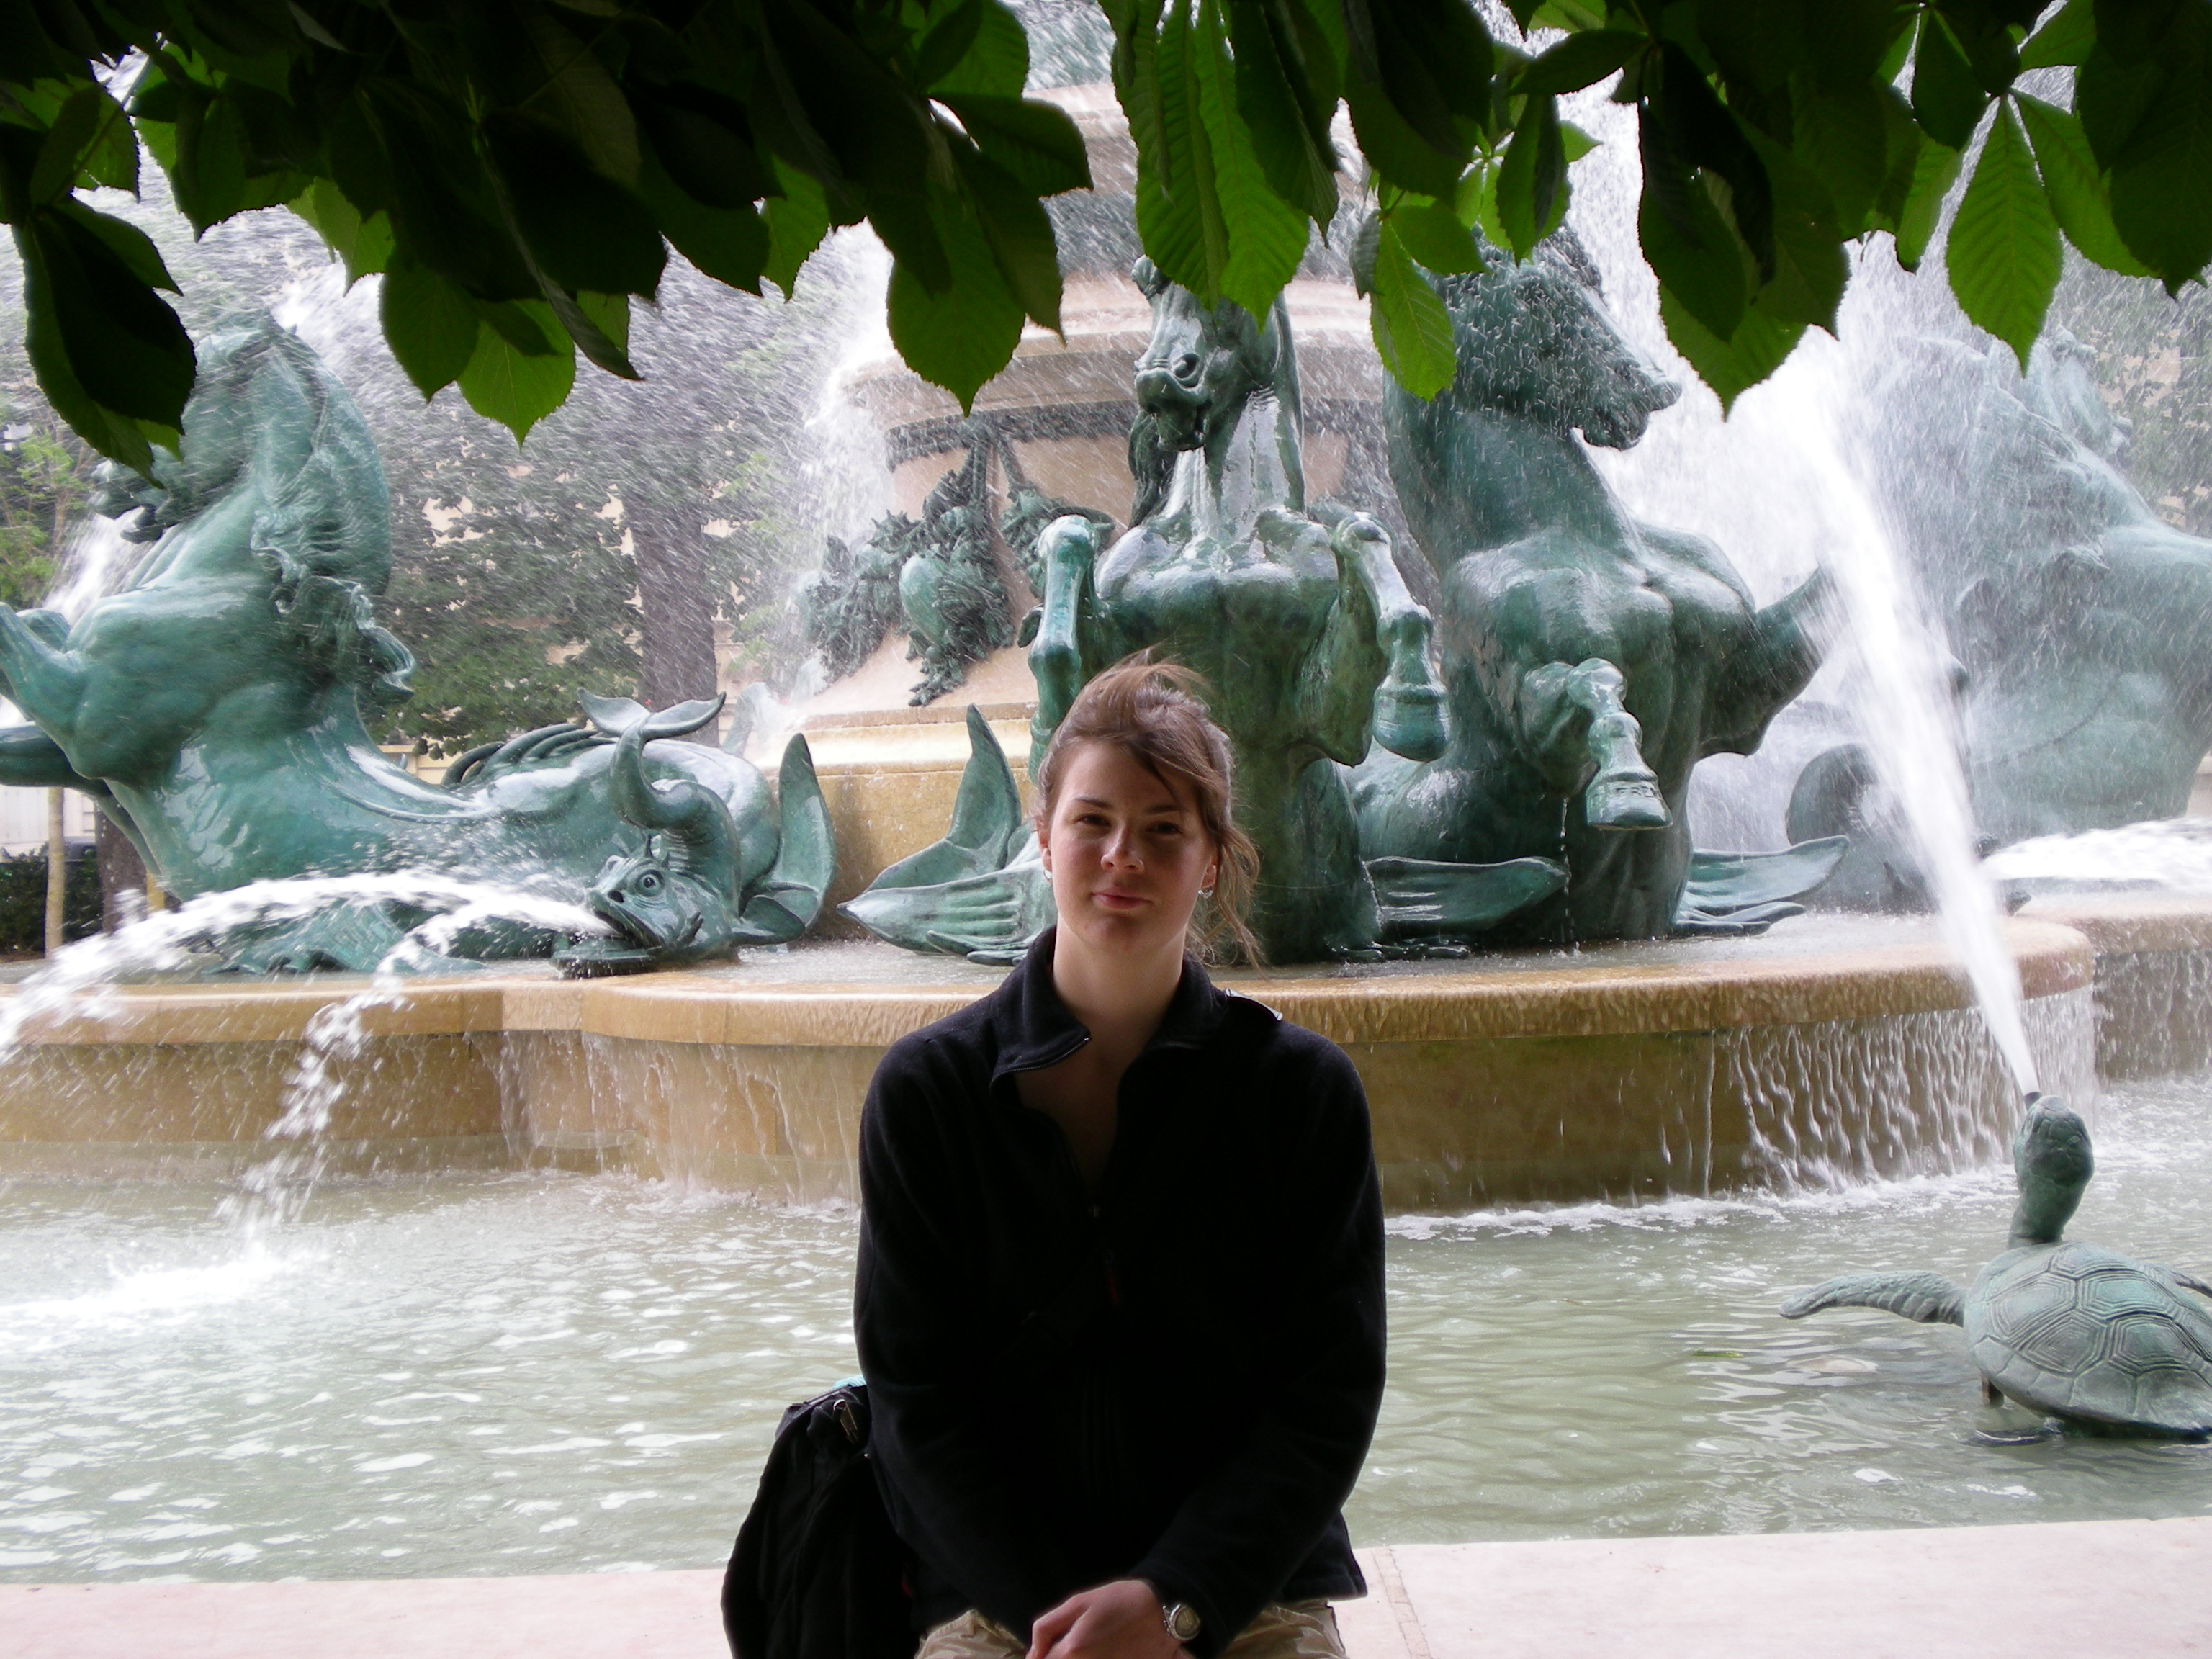
\includegraphics[width=0.6\textwidth]{images/method/tortoise_seaturtle.jpg}
    \caption{
        An image with at least one mislabelled concept: The fountain statue is labelled as both ``Tortoise" and ``Sea turtle"; it cannot be both. 
    }
\end{figure}

In this experiment, there are no links between any concepts to any entities in the real world. The embeddings are learned completely independently of their associated labels and are numbered by the index they occur in the co-occurrence data. For example, the first index in the Open Images co-occurrence matrix is ``Sprenger's tulip", which has label \texttt{/m/0100nhbf}, but neither of these strings (the human name or the machine ID) are used anywhere in the learning system. Any meaning ascribed to relationships between embeddings must be inferred from re-mapping the indexes back to the concept names. If the algorithm generates embeddings for concepts with indexes 15268 and 5296 that are nearest neighbours in embedding space, we will not know until we perform this re-mapping that the concepts 15268 and 5296 are ``Coffee" and ``Tea" (in which case they are related), or that they are ``Sprenger's tulip" and ``Ferret" (in which case they are not related). 

The co-occurrence matrices for the Open Images and AudioSet datasets, as well as the concept name to label mapping files, make up the dataset for these experiments. This dataset should represent the statistical distribution of co-occurrence of concepts in the two modalities. The co-occurrence for a pair was incremented by 1 if both items in the pair were present in an image or audio clip. The raw data files also contained a confidence score for the degree of certainty of the labelling, but this was not used. 

\section{Embedding choice: Probabilistic GloVe}

The dimension of the co-occurrence matrices is high, particularly the Open Images matrix which is 19996 by 19996 (AudioSet is a more manageable 526 by 526). However, they are extremely sparse, and this is ideal for dimensionality reduction. Since the  GloVe learning algorithm uses only the non-zero items in the co-occurrence matrix, it is a particularly efficient choice. Also, its computational complexity depends on the number of such non-zero items rather than on the size of the co-occurrence matrix. It produces reasonable clustering, where concepts that are close in embedding space are also close in semantic space. %\cite{pennington2014glove} found that the embedding space produced by this algorithm gave state-of-the-art accuracies on word analogy tests. 
GloVe embeddings are also stable, by the metric used in \cite{WordEmbeddingStability}- the amount of overlap between nearest neighbours of an embedding for different runs. As the GloVe embedding is trained by stochastic gradient descent, the embeddings resulting from different random seeds will be different.

We modify this model to be probabilistic.  The probabilistic/deterministic distinction refers not to the learning algorithm (as any algorithm trained by stochastic gradient descent will have a probabilistic component), but to the embedding representation. The original GloVe embeddings are represented by point estimates for each concept (thus a single vector for each concept); in our implementation, each probabilistic embedding represents a multivariate Gaussian distribution with independent dimensions (diagonal covariance matrix). The motivation for this is the hope that the variances learned will give us some knowledge of the degree of confidence we can have in each embedding, and also that learning two parameters for each embedding will help with alignment by providing more information for disambiguation. 

A probabilistic embedding is a sample from the following distribution:
\begin{equation*}
    \mu + \sigma \N(0, 1)
\end{equation*}

Both $\mu$ and $\sigma$ are learned parameters. In practice, $\sigma$ is further parametrised as follows, to enforce positivity:

\begin{equation*}
    \sigma = \ln (1 + \exp (\rho))
\end{equation*}

Therefore the full equation is:

\begin{equation*}
\label{eq:stochemb}
    \mu + \ln (1 + \exp(\rho)) \cdot \N(0, 1)
\end{equation*}

\subsection{Implementation}

The probabilistic version of the GloVe algorithm was implemented in Python using the PyTorch \cite{pytorch}, PyTorch Lightning \cite{pytorchlightning} and Pyro \cite{pyro} libraries. A custom neural network layer was implemented which took as input a co-occurrence matrix, and learned probabilistic GloVe embeddings by backpropagation through the loss function. Each mini-batch represented a random sampling of the rows and columns of the co-occurrence matrix, with all rows and columns being used over the course of one training epoch. 

The GloVe loss function from \cite{pennington2014glove} is reproduced here:

\begin{equation}
\label{eq:gloveloss}
\begin{split}
L_{glove} &= \sum_i \sum_j f(X_{ij}) (\vecw_i^T \vecw_j + b_i + b_j - \log X_{ij})^2\\
f(x) &= \begin{cases}
(x/x_{max})^{\alpha}\spaced{if} x \le x_{max}\\
1\spaced{otherwise}
\end{cases}
\end{split}
\end{equation}

\begin{itemize}
    \item The values of hyperparameters $\alpha = 0.75$ and $x_{max} = 100$  are taken from the original paper, \cite{pennington2014glove}. 
    \item The $\vecw_i$ and $\vecw_j$ are samples of the current probabilistic embeddings represented by equation \ref{eq:stochemb}. 
    \item The $X_{ij}$ are co-occurrence statistics of the $i$th and $j$th concept.
\end{itemize}

The Pyro library provides backpropagation through the random sampling, as described in \cite{deeplearninggoodfellow} (section 20.9). The next section describes how these probabilistic embeddings were verified. 

\subsection{Validation}

The probabilistic embeddings were validated as follows:

\begin{itemize}
    \item Train embeddings learned from Open Images and AudioSet co-occurrence data individually without regard for alignment between domains.
    \item For each run of each domain, set a different random seed. 10 seeds were used to get 10 instances of embeddings per domain.
    \item The following learning parameters were used:
    \begin{itemize}
        \item Embedding dimension of 6. This choice was heuristic: the test implementation of GloVe embeddings implemented in PyTorch had 1 million unique tokens and dimensionality of 300, to keep the same ratio of effective tokens to dimensionality, 6 was the closest integer. 
        \item Mini-batch size of 500.
        \item The Adam \cite{kingma2017adam} optimiser, with learning rate 0.01.
        \item 250 epochs of training for Open Images and 2000 epochs for AudioSet. This was enough to ensure convergence of the GloVe loss decreasing to asymptotic levels. 
    \end{itemize}
    \item No hyperparameter tuning was done; as this is not a supervised learning problem, we measure convergence only by the decrease in GloVe loss (equation \ref{eq:gloveloss}) as there is no validation set to cross-check with. 
\end{itemize}

This resulted in 10 sets of probabilistic embeddings for each domain. These embeddings are stochastic in two senses; one source is stochasticity in the learning algorithm leading to 2 runs with different seeds converging to different mean embeddings, and the other is caused by each embedding being a sample from a multivariate Gaussian distribution. 

It is interesting that AudioSet needed many more epochs to converge. This is consistent with an earlier point mentioned in \cite{GOLDSTONE2002295} that systems with more concepts are easier to learn as they are more constrained. 

\newpage
\subsubsection{Clustering}
As a sanity check, the t-SNE (t-Distributed Stochastic Neighbor Embedding, \cite{tsne}) algorithm was  used to reduce the dimensionality of the embeddings from 6 to 2, and the resulting points plotted for the top 300 most frequent concepts in each domain (measured by number of occurrences in images or audio clips). As we expected, there are clearly visible concept clusters.  While t-SNE adds a further level of stochasticity during the dimensionality reduction process, two runs of t-SNE on the same input data with the same t-SNE random seed set, will produce the same result. Therefore, we can assume that the stochasticity introduced by t-SNE is accounted for. 

This is a qualitative analysis only intended to confirm that the implementation is correct and converges to embeddings that have meaningful semantic relationships. This technique of using t-SNE to verify embedding quality is used in similar experiments, for example, \cite{CoocurrenceVisionLanguage2021}. 

\begin{figure}[H]
\label{fig:gloveclusters}
    \centering
    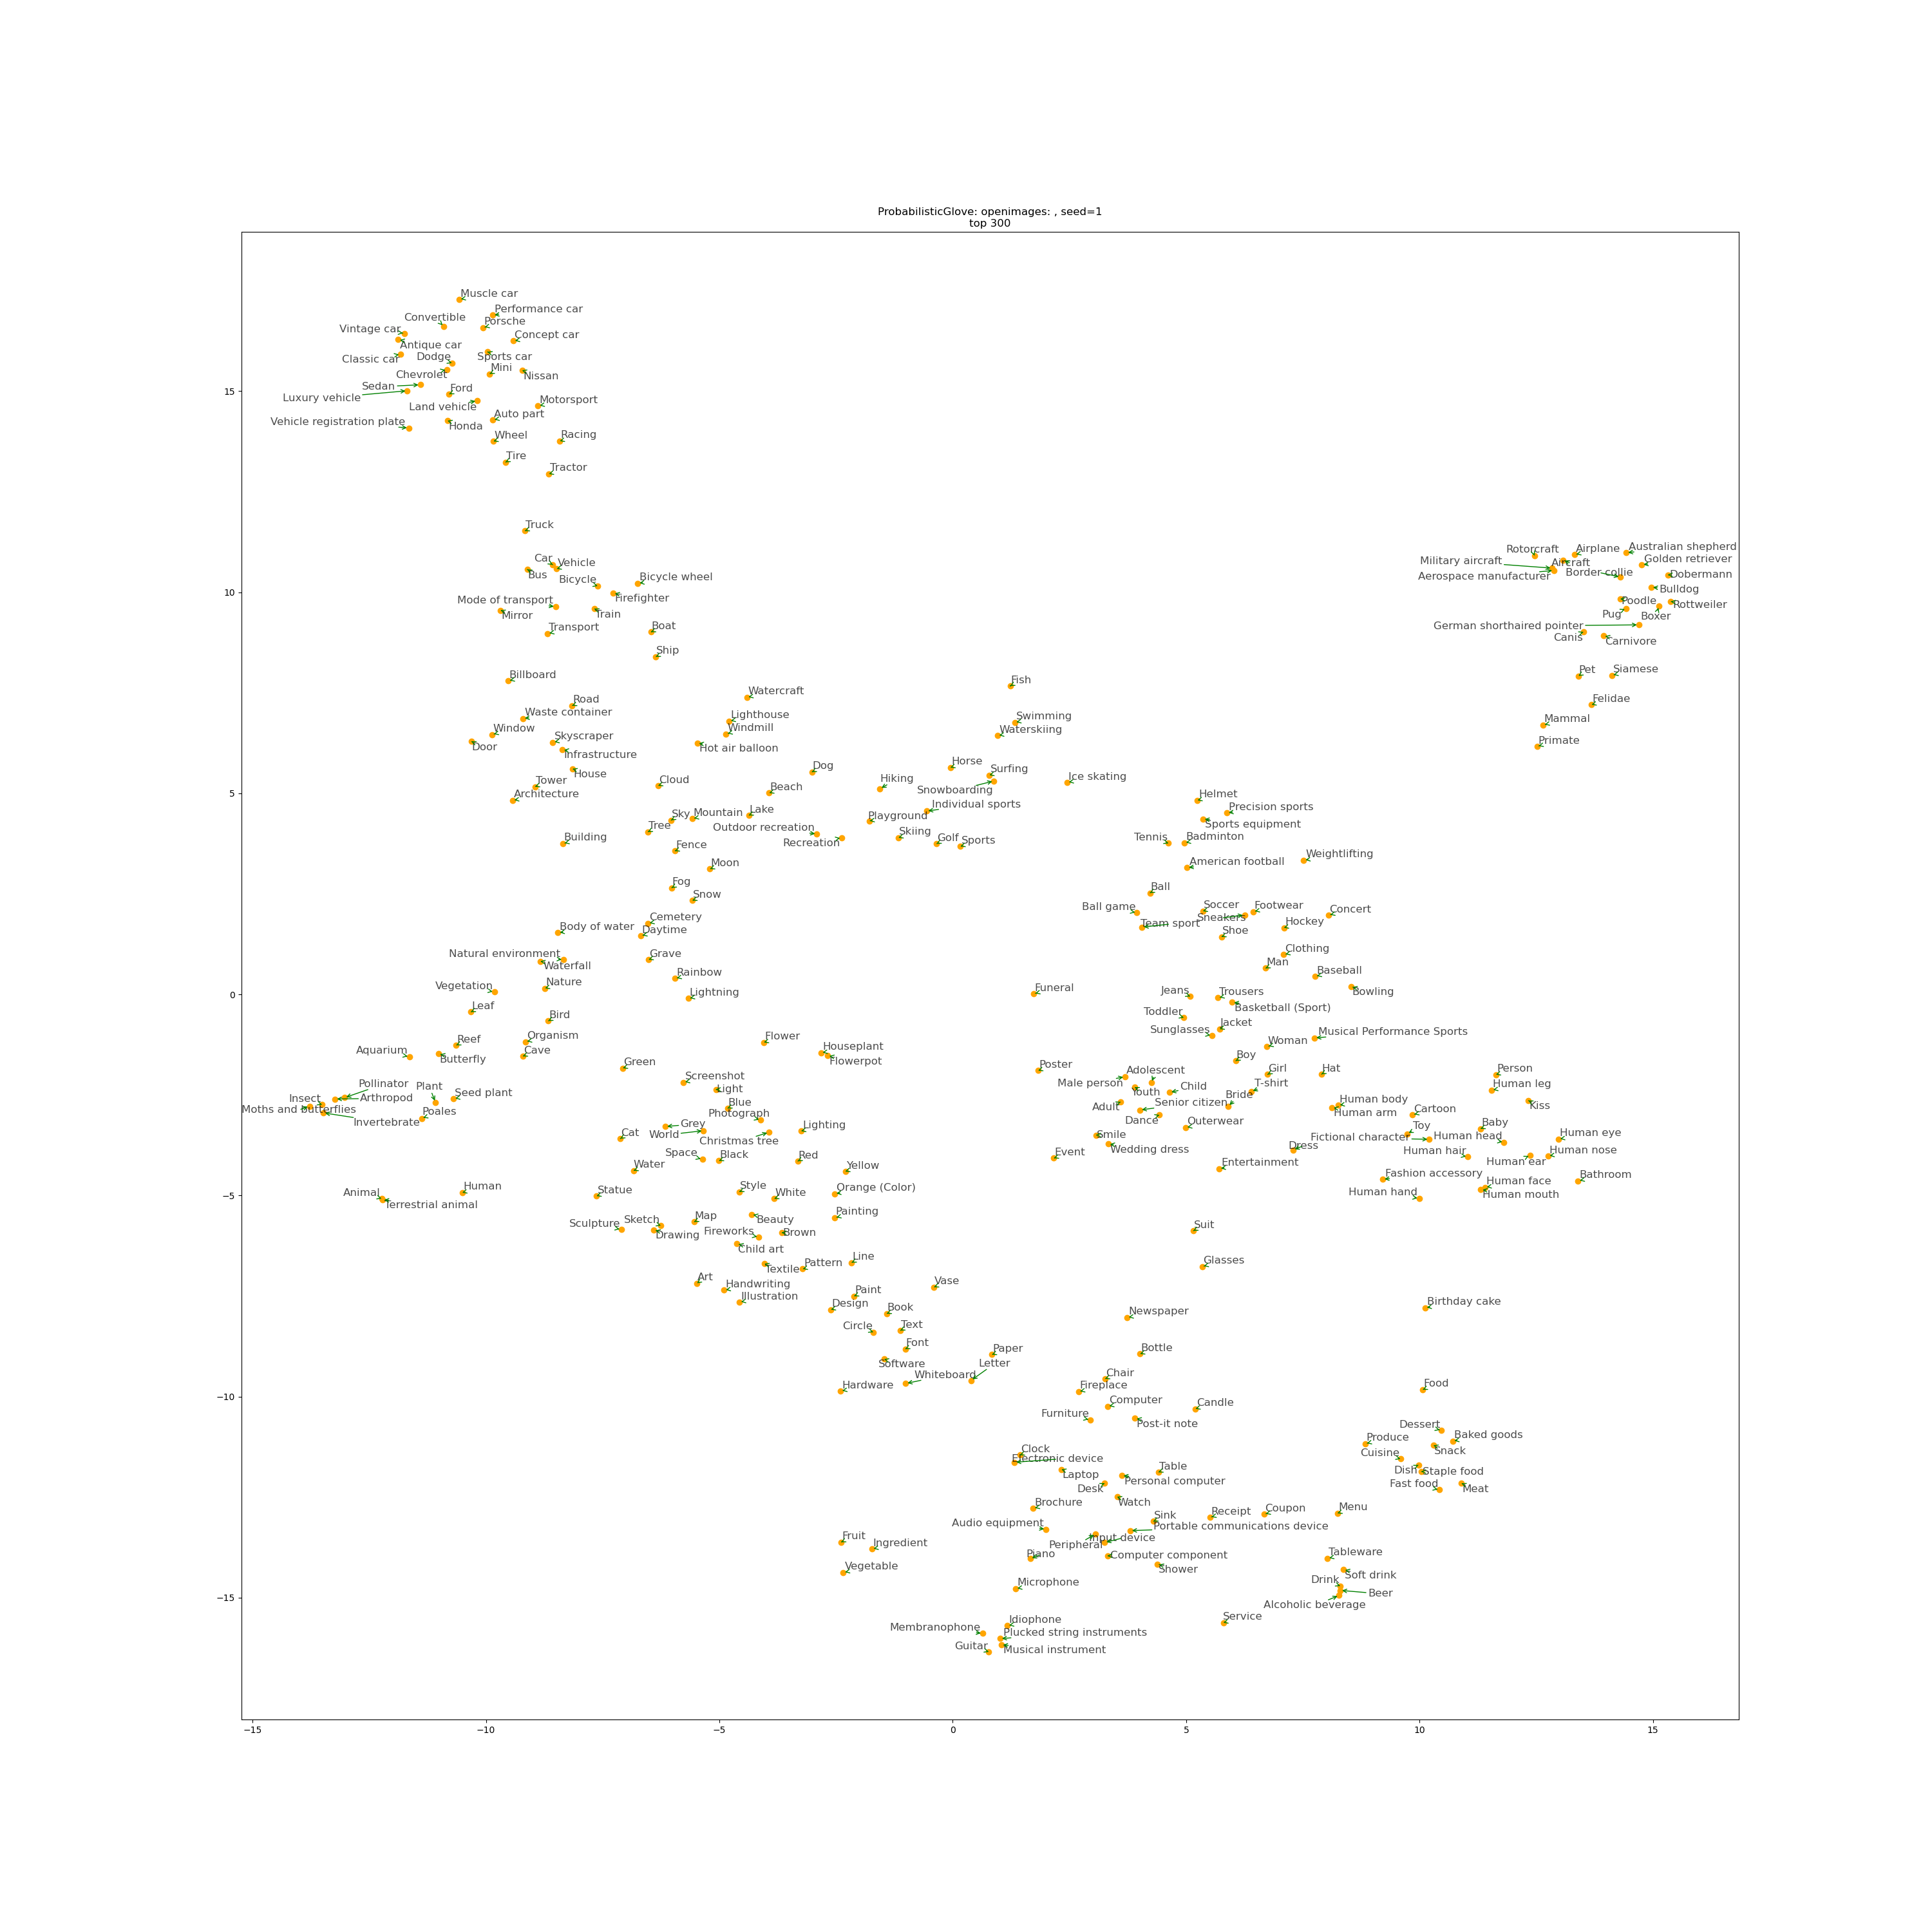
\includegraphics[width=\textwidth]{images/method/probabilistic_independent/top300_tsne_openimages__ProbabilisticGlove_1.png}
    \caption{
        Open Images top 300 most common concepts. There are clearly visible clusters corresponding to, amongst other things, different types of dog, different types of vehicle, and different types of human body part.
    }
    % generated by inspect_results.py 
\end{figure}

\begin{figure}[H]
    \centering
    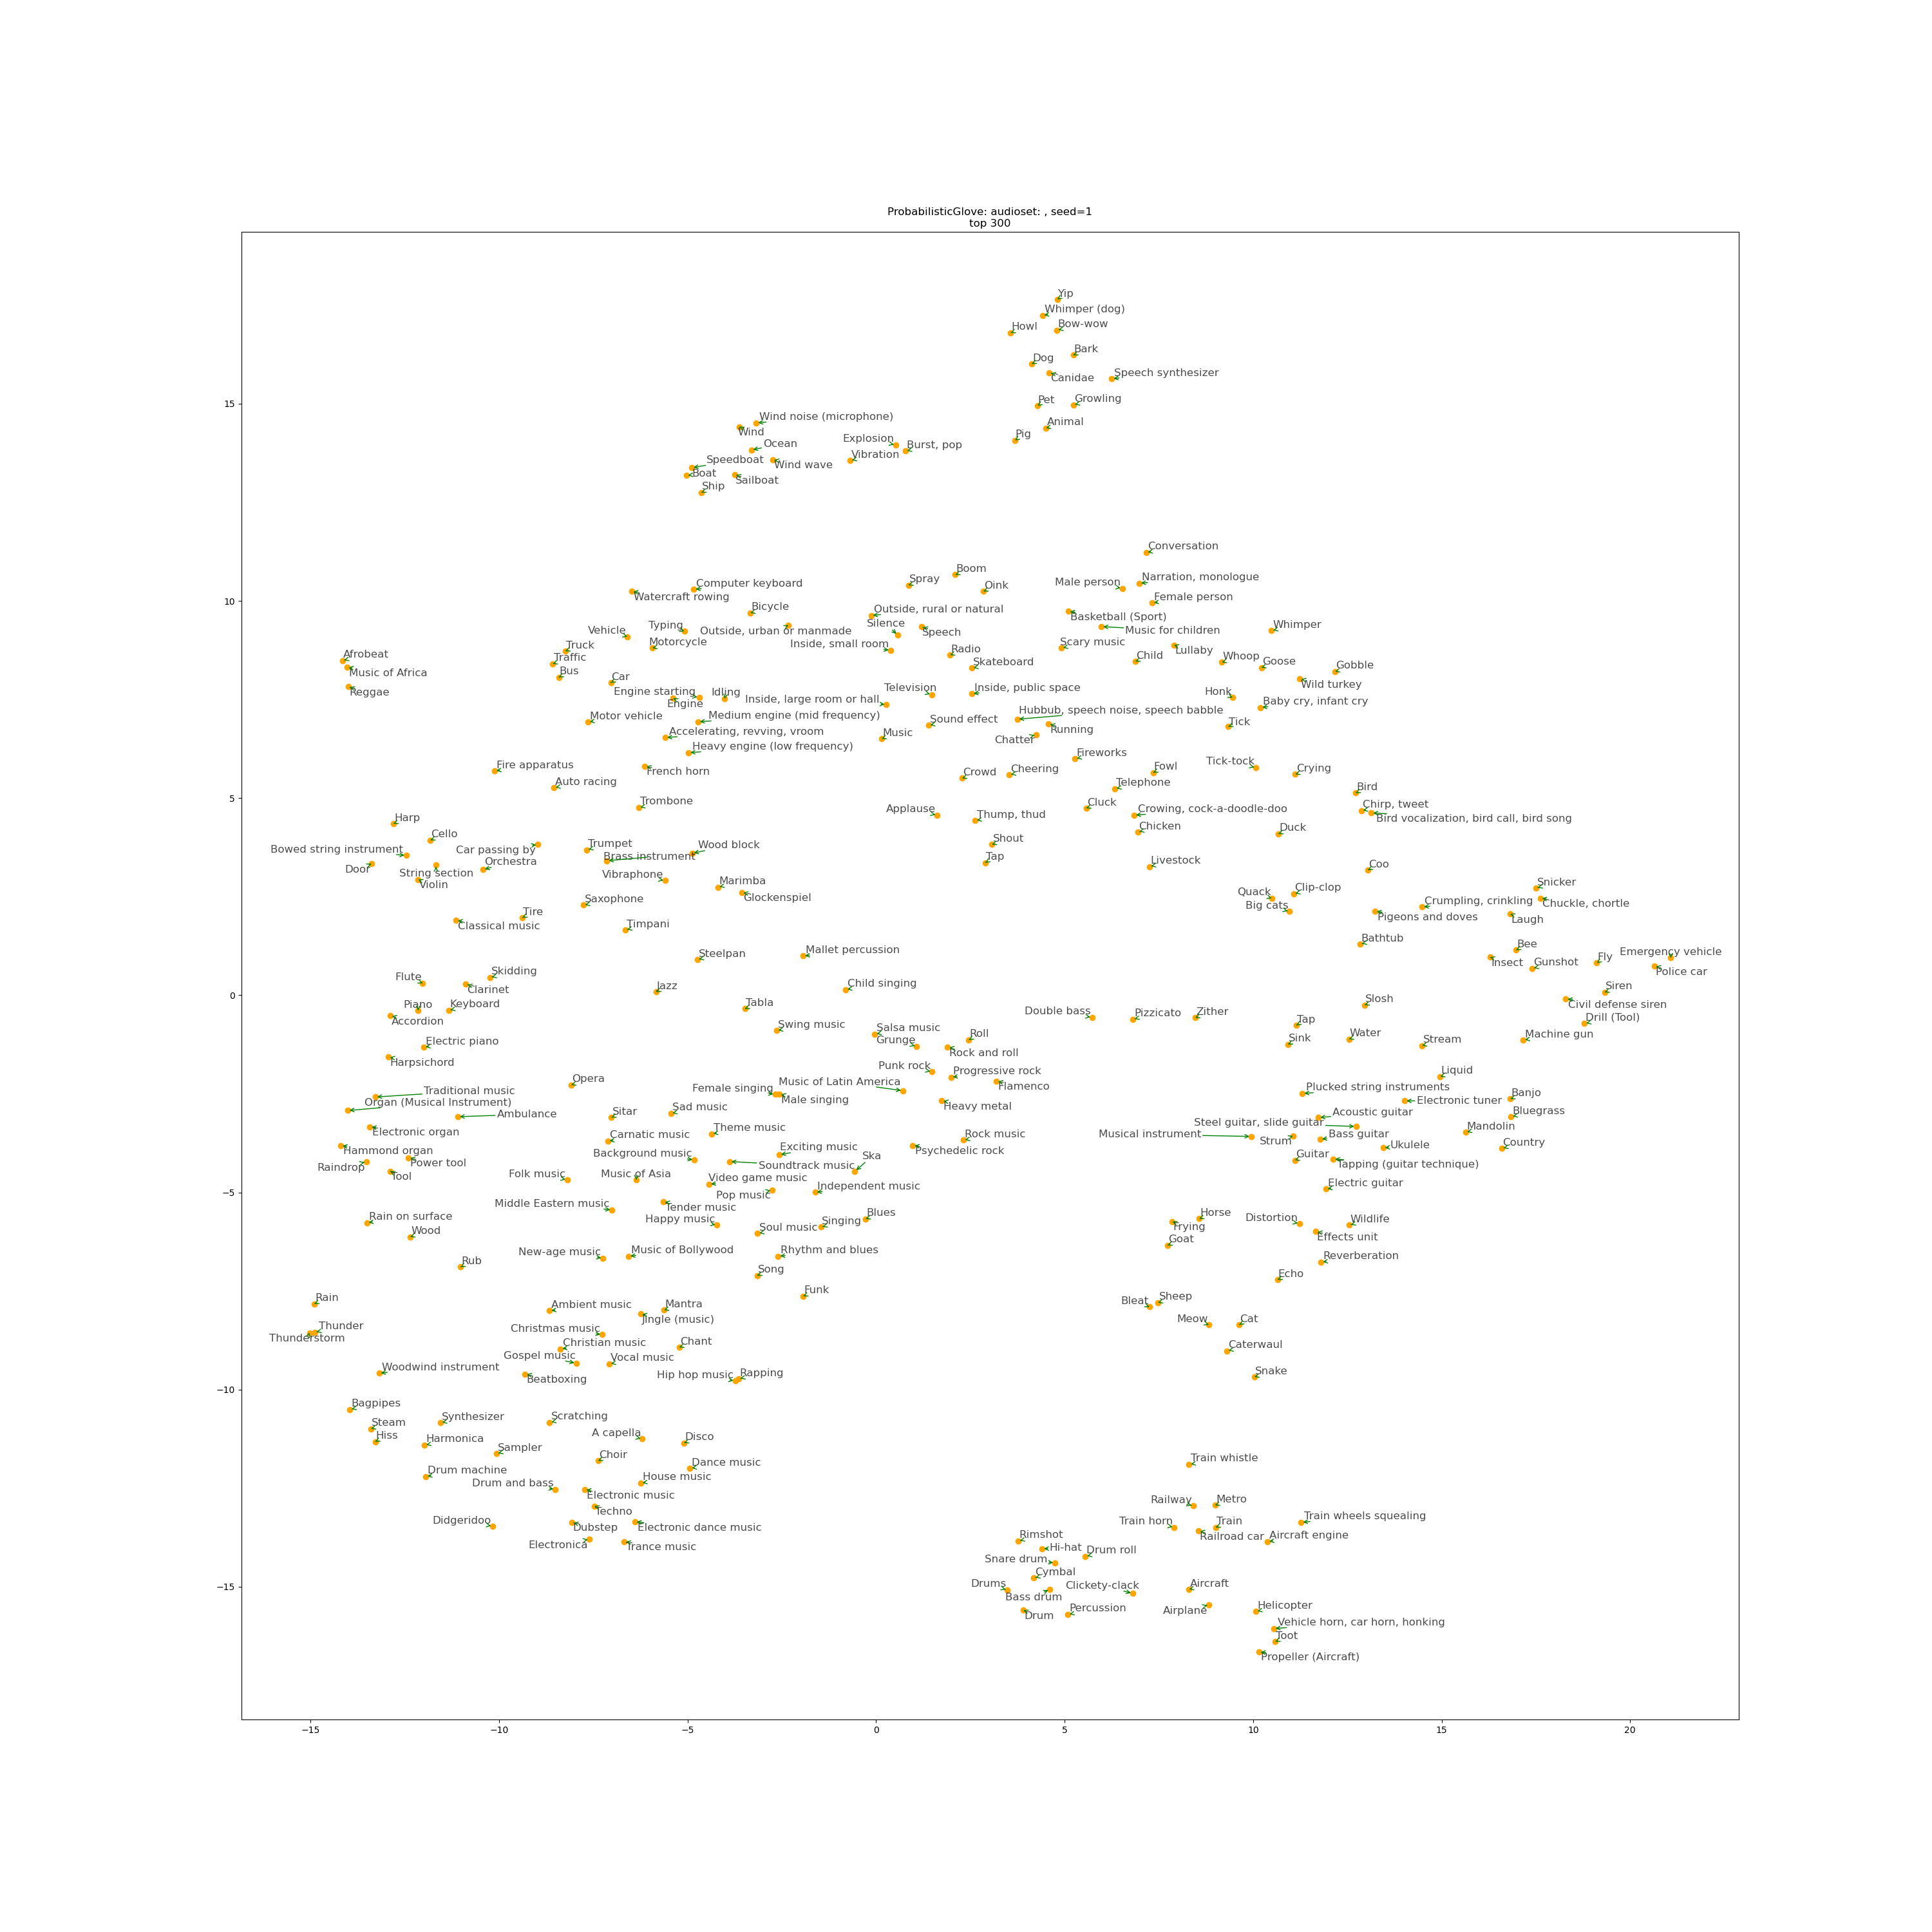
\includegraphics[width=\textwidth]{images/method/probabilistic_independent/top300_tsne_audioset__ProbabilisticGlove_1.png}
    \caption{
        AudioSet top 300 most common concepts. Again there are clearly visible clusters comprising, for example, sounds made by water, sounds made by percussion instruments, and sounds made by dogs. 
    }
    % generated by inspect_results.py 
\end{figure}

The following plots of the Open Images top 300 concepts (by frequency) t-SNE plots annotated to show some of the clusters, for random seeds 1 and 2, show that roughly the same concepts cluster for each run. They also reveal a characteristic of our alignment problem: The cluster arrangements relative to each other across runs are not consistent. Ideally, we would like the different clusters to have the same spatial arrangement across runs. As described in \cite{SHEPARD19701}, we would like to identify second order isomorphisms in the data; not just the clusters, but the relationships between the clusters. The variability from run to run suggests that the available data does not uniquely identify a single system of second-order isomorphisms. We attempt to inject additional constraints in a later section.

\begin{figure}[H]
    \centering
    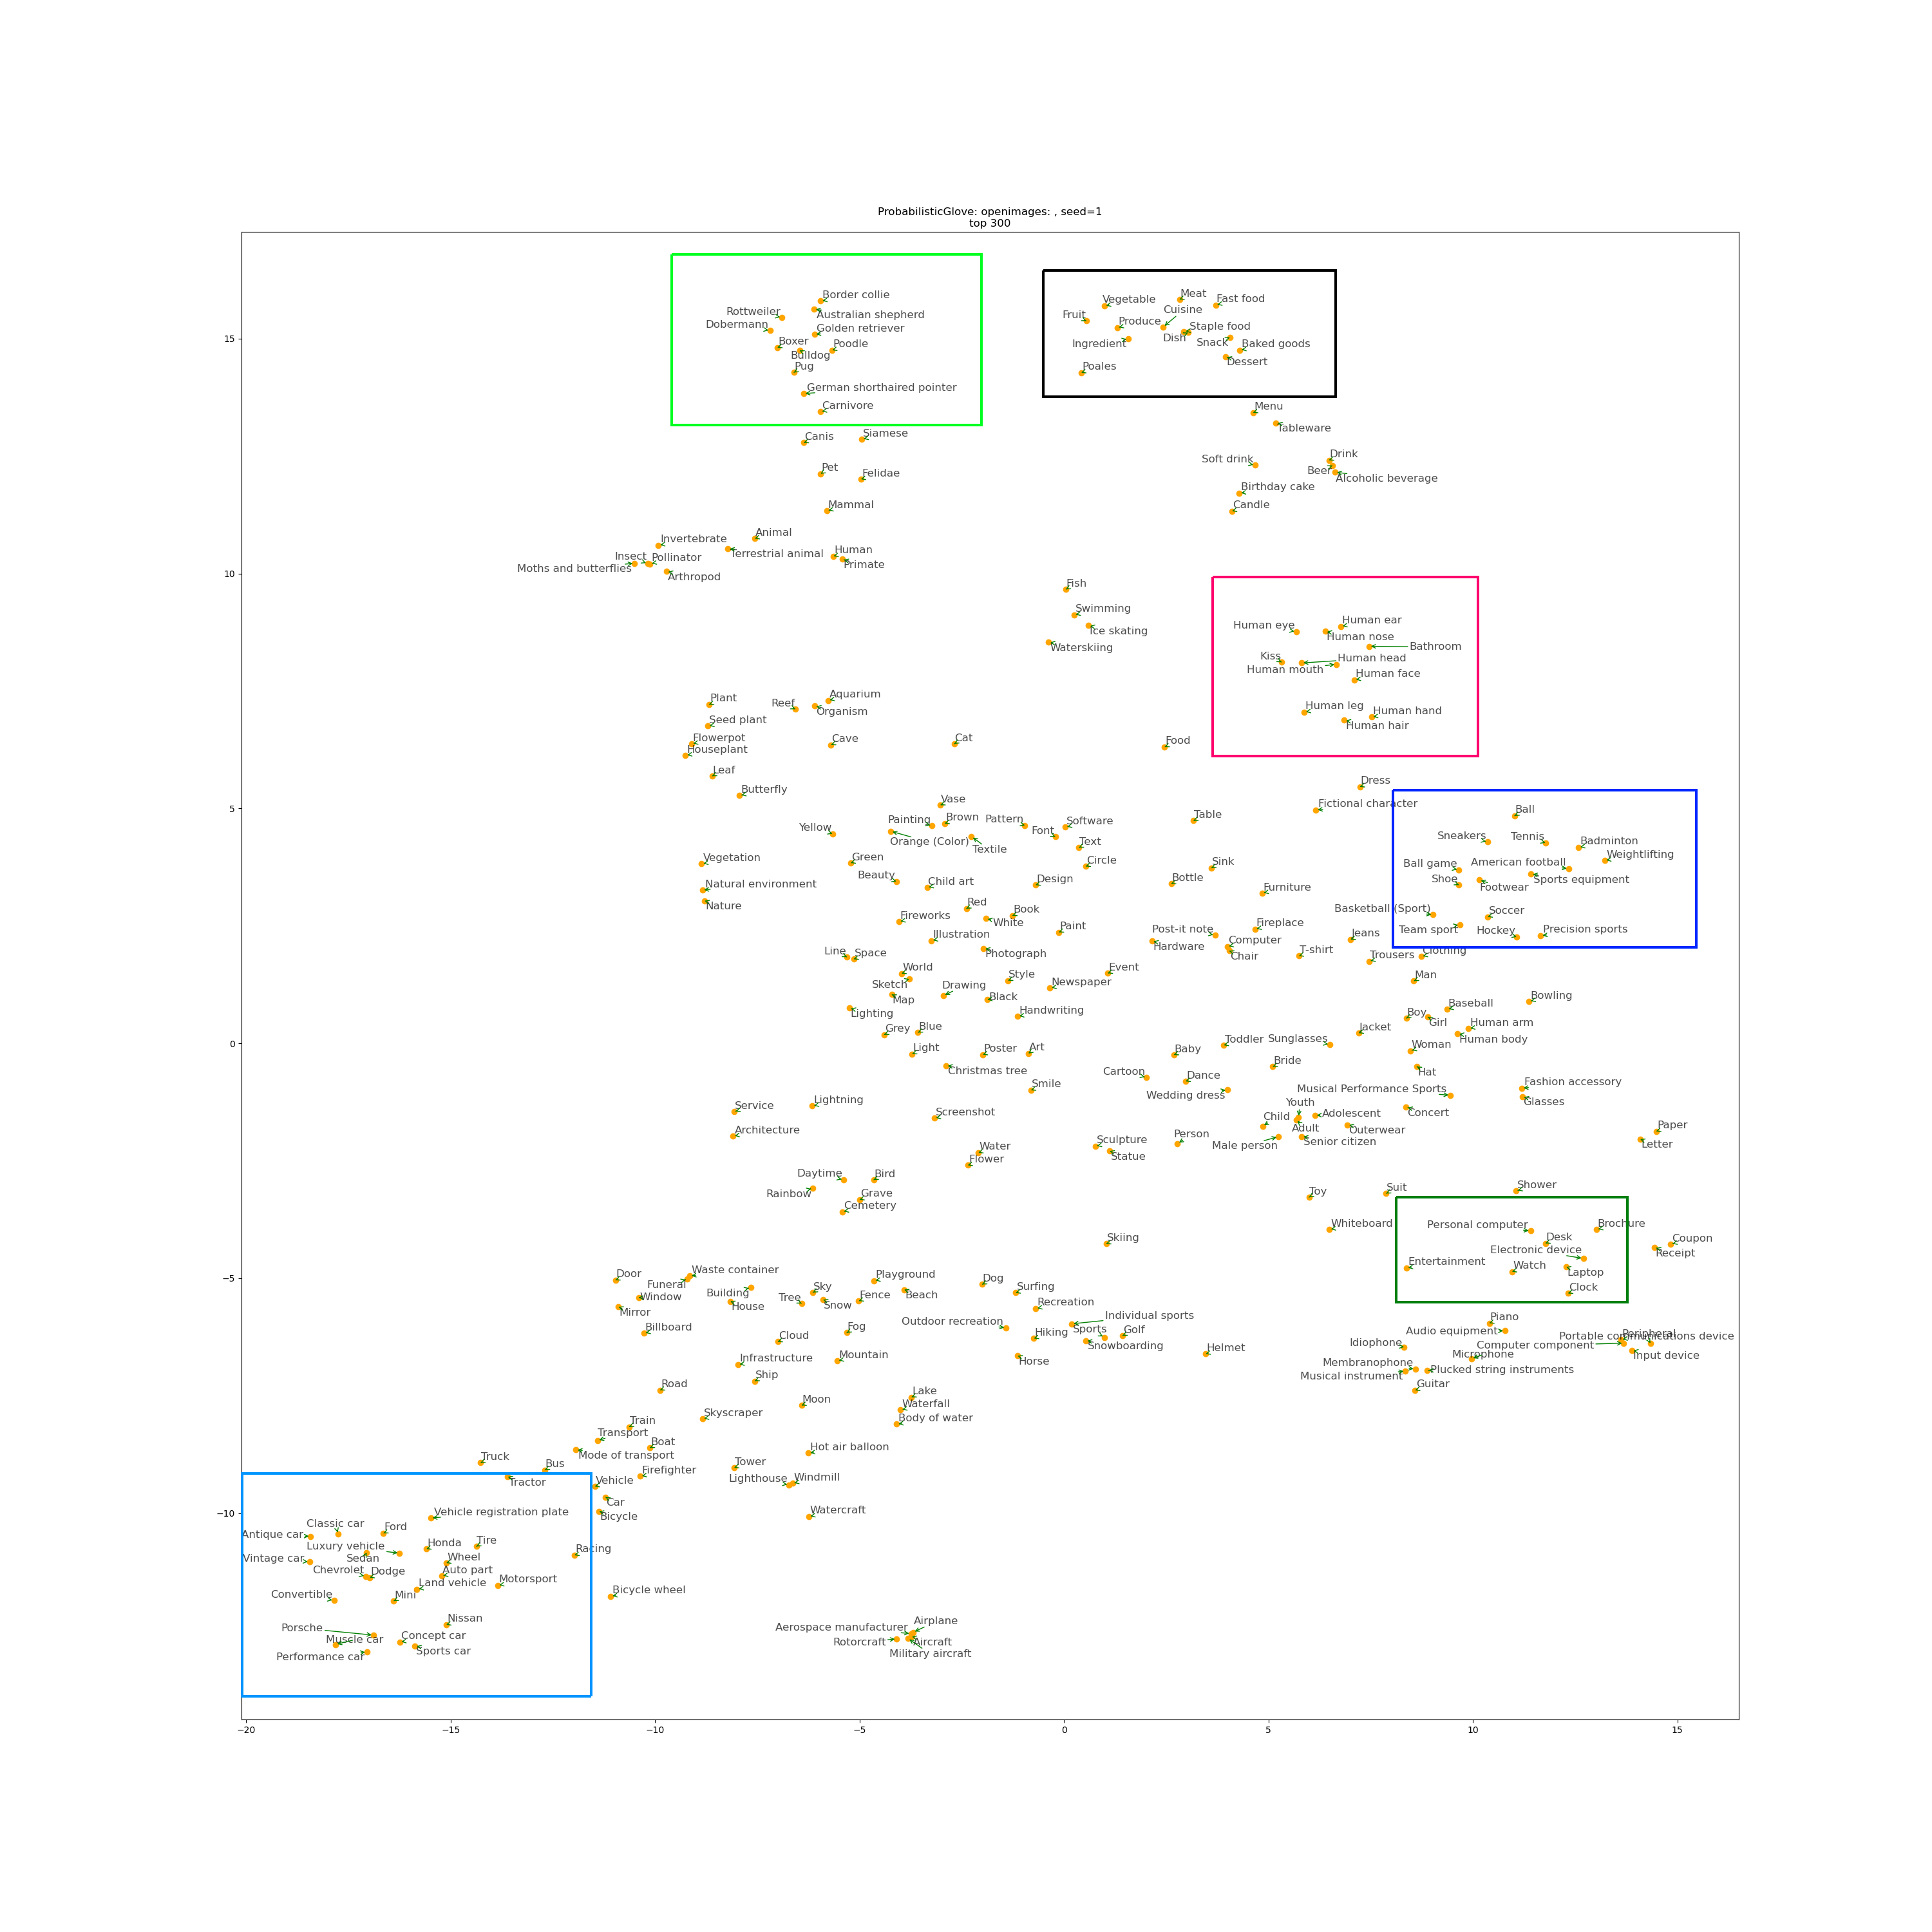
\includegraphics[width=\textwidth]{images/method/probabilistic_independent/top300_tsne_openimages__ProbabilisticGlove_1_clusters.png}
    \caption{
        Coloured boxes indicate clusters 
    }
    % generated by inspect_results.py 
\end{figure}

\begin{figure}[H]
    \centering
    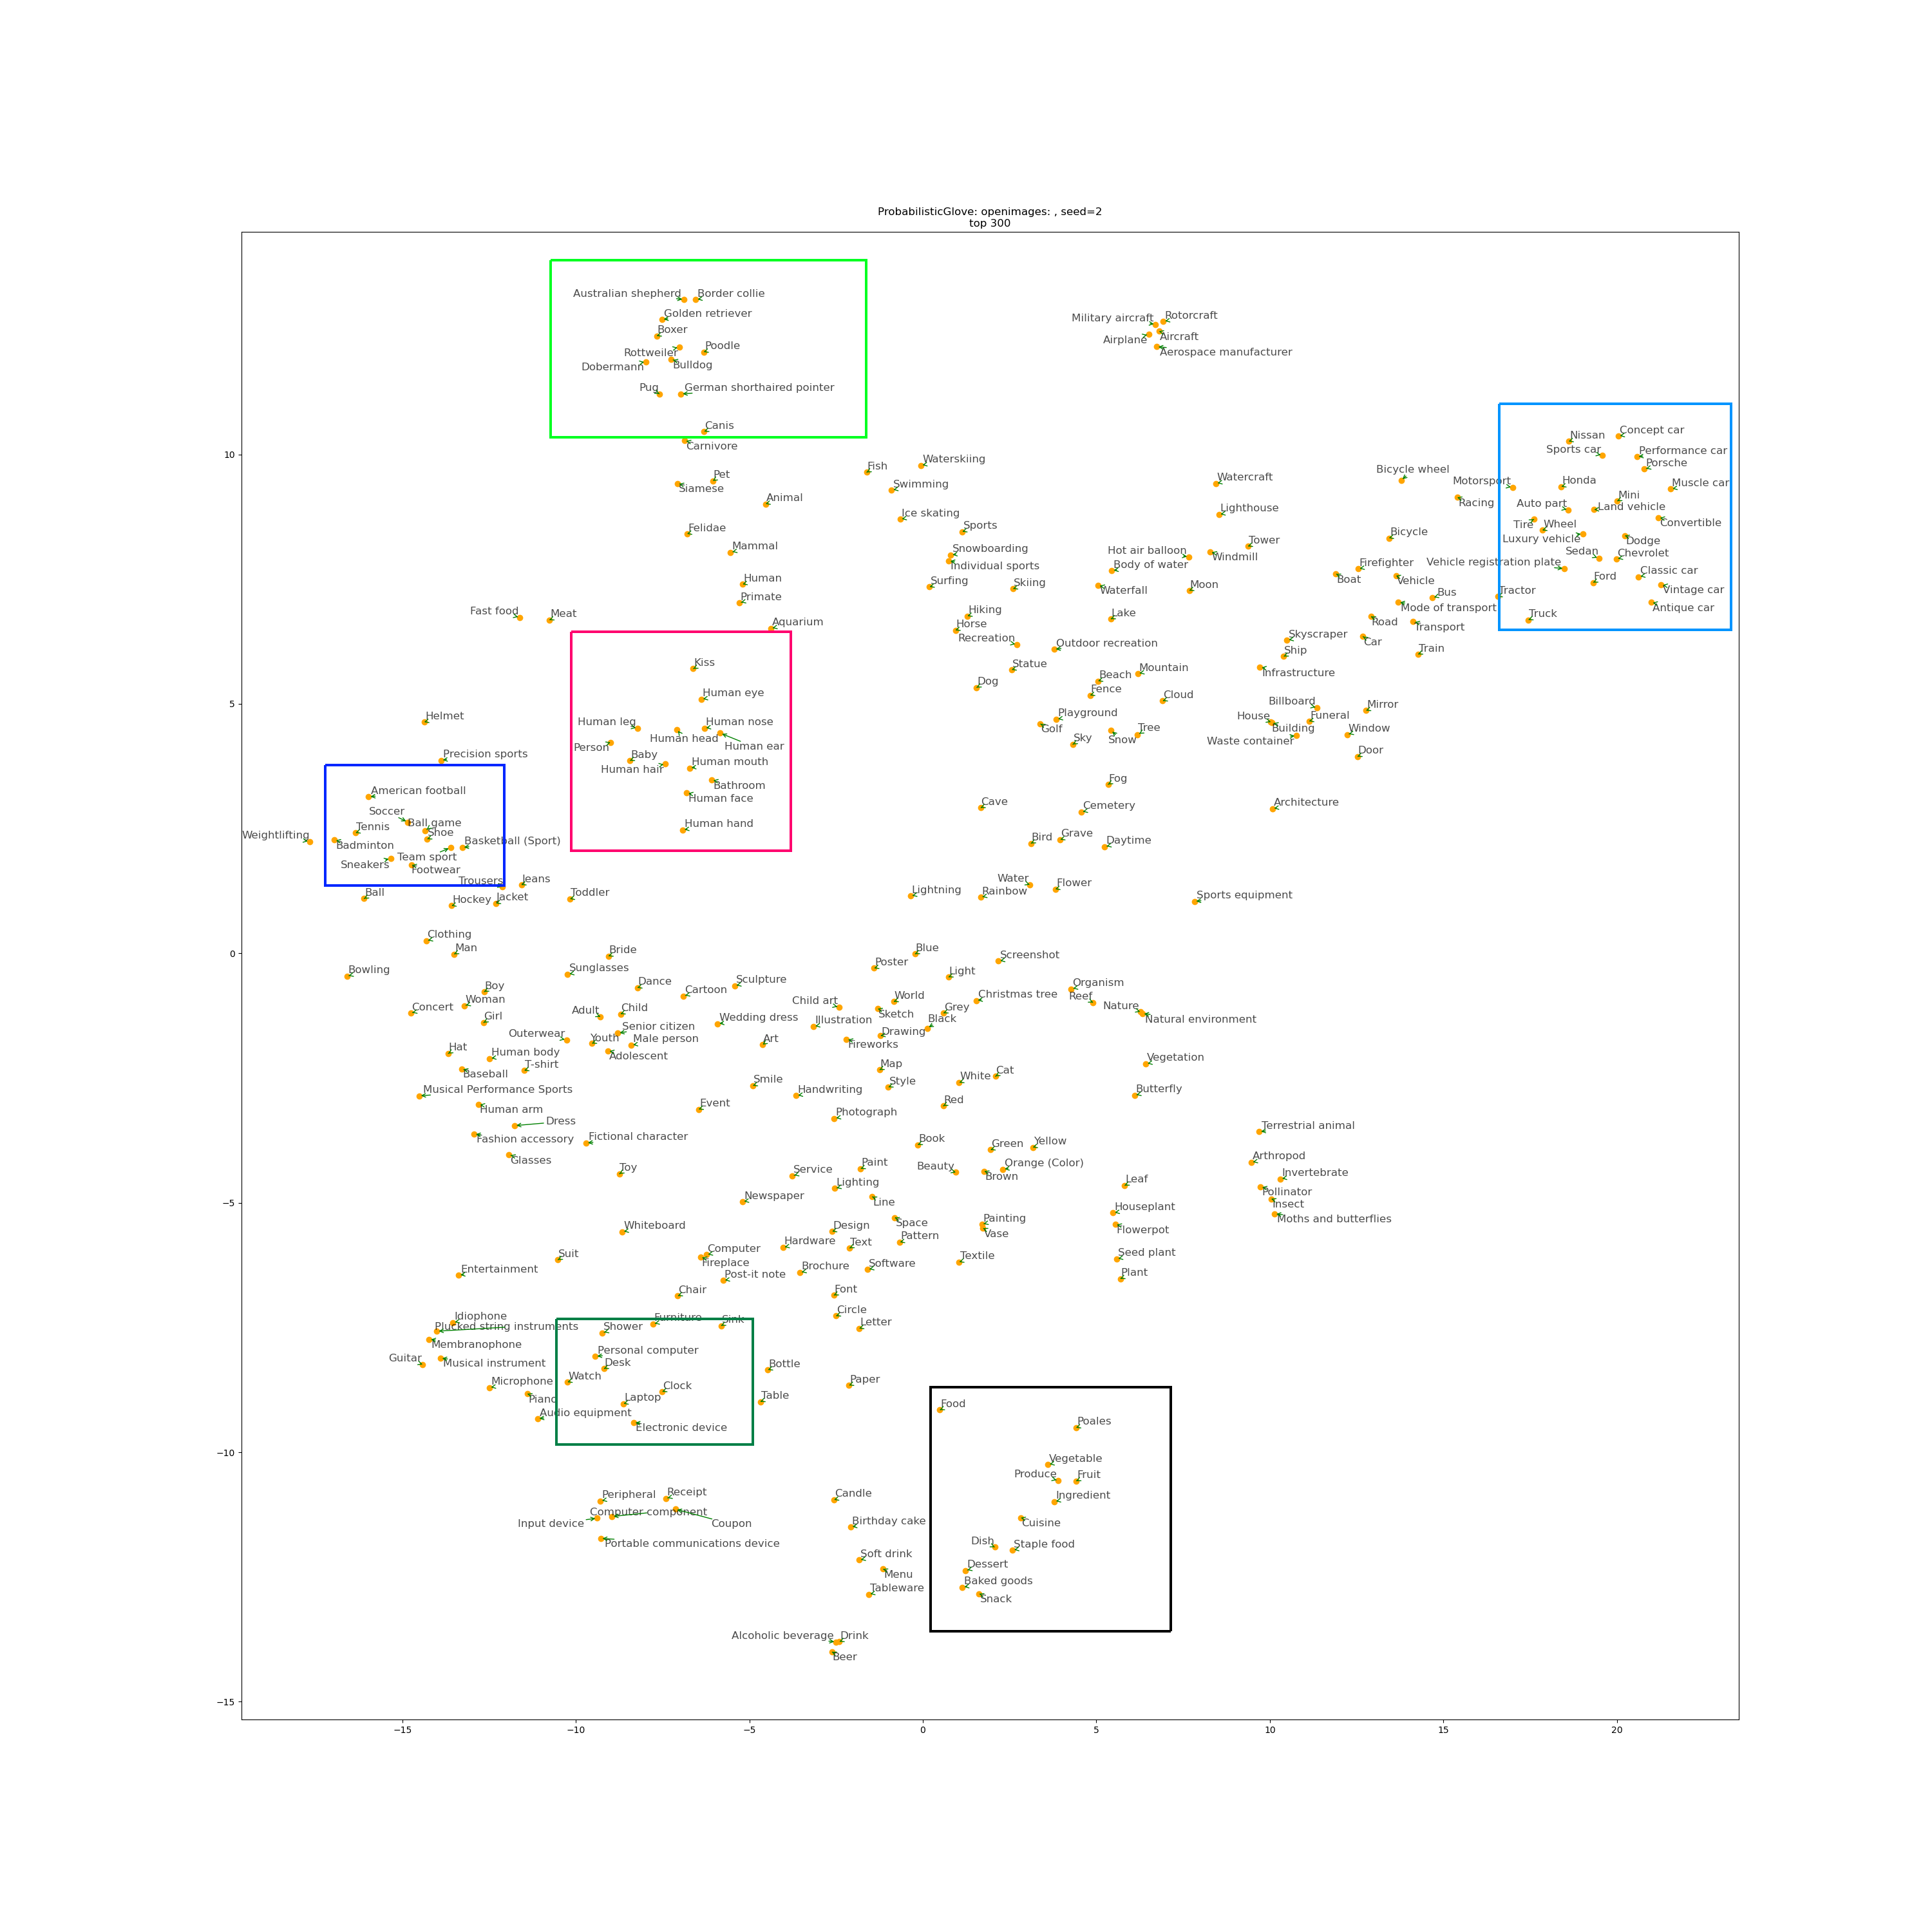
\includegraphics[width=\textwidth]{images/method/probabilistic_independent/top300_tsne_openimages__ProbabilisticGlove_2_clusters.png}
    \caption{
        The same clusters are in different locations in embedding space compared to the previous run, and their orientation relative to each other is different; it is not a simple rotation and stretch of the clusters. Although t-SNE introduces more stochasticity, both t-SNE runs were done with the same t-SNE random seed set, which is known to generate the same output if given the same inputs. 
    }
    % generated by inspect_results.py 
\end{figure}

\newpage
\subsubsection{Learned parameters of the probabilistic embeddings}

We also examine the learned means and variances, $\mu$ and $\sigma = \ln(1 + \exp(\rho))$, of each embedding. 

This is done as follows for each domain (Open Images and AudioSet separately):

\begin{itemize}
    \item The dot products are calculated between the learned $\mu$ (the mean of the stochastic embeddings) for every pair of concepts. The stochastic embeddings can be thought of as distributions about a mean, where the mean would be the embedding learned in the deterministic case. 
    \item This gives a similarity matrix between each embedding and itself, for each seed. 
    \item The correlation between the values of each run's similarity matrix with every other run was computed, and the mean value taken. A high value should indicate that over runs with different seeds, the similarity of a given pair of concepts is consistent. If a pair is similar in one run, it should be similar in another run and vice versa. 
    \item The average cross-correlation was $ 0.412 \pm 0.045$ for AudioSet and $0.590 \pm 0.049$ for OpenImages. 
    \item The same procedure was done above, but instead of using the learned $\mu$ for every pair of concepts, 100 samples of each concept embedding were taken, and 100 similarity matrices calculated using those samples, to get a mean similarity matrix based on sampling. The same cross-correlation was computed, which yielded the values $ 0.412 \pm 0.044$ for AudioSet and $0.589 \pm 0.049$ for OpenImages (the numbers are indeed very similar). 
% /home/petra/spond/spond/experimental/glove/results/audioset/ProbabilisticGlove/audioset_analytics.hdf5
% /home/petra/spond/spond/experimental/glove/results/openimages/ProbabilisticGlove/openimages_analytics.hdf5
\end{itemize}

There is a reasonable correlation between the similarity of pairs between runs over both domains. The similarity between runs is higher for AudioSet; there are fewer concepts in this domain so this is expected. 

The variances were examined by analysing the entropy of each embedding. Since each embedding is a multivariate Gaussian with a diagonal covariance matrix:

\begin{equation*}
\begin{split}
H(x) &= \frac{1}{2} \ln |\Sigma| + \frac{D}{2}(1 + \ln(2 \pi))\\
&= \frac{1}{2} \ln \prod_{i=1}^D \sigma_i + \frac{D}{2}(1 + \ln(2 \pi))\\
\end{split}
\end{equation*}

with $\sigma_i$ being the variance for dimension $i$. 
 
Distributional plots of the entropies will give us information about the algorithm's stability over different runs:

\begin{figure}[H]
\label{fig:entropyindependent}
    \centering
    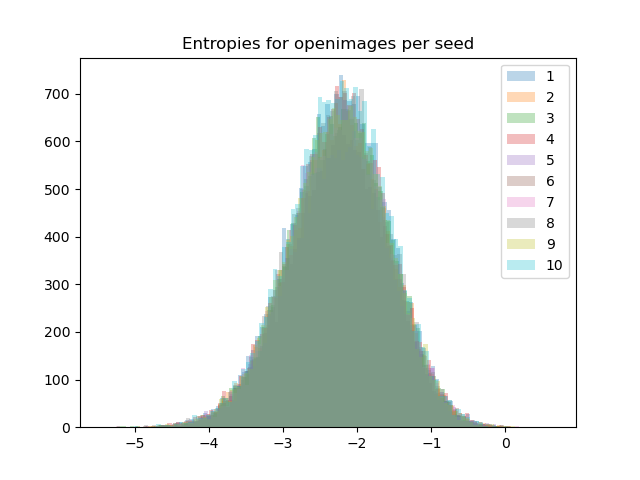
\includegraphics[width=0.45\textwidth]{images/method/probabilistic_independent/openimages_entropies.png}
    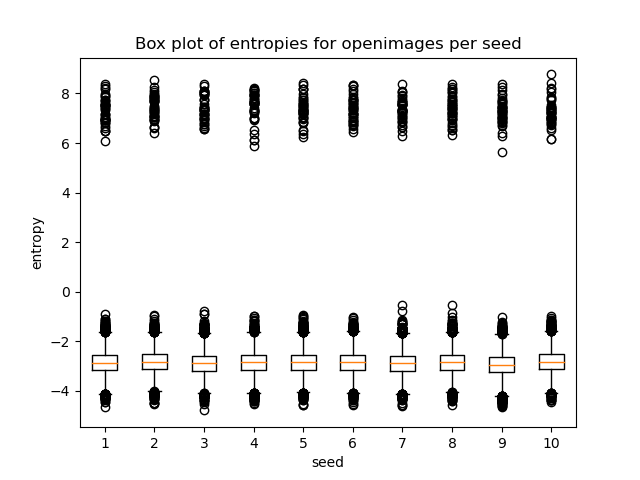
\includegraphics[width=0.45\textwidth]{images/method/probabilistic_independent/openimages_entropies_box.png}
    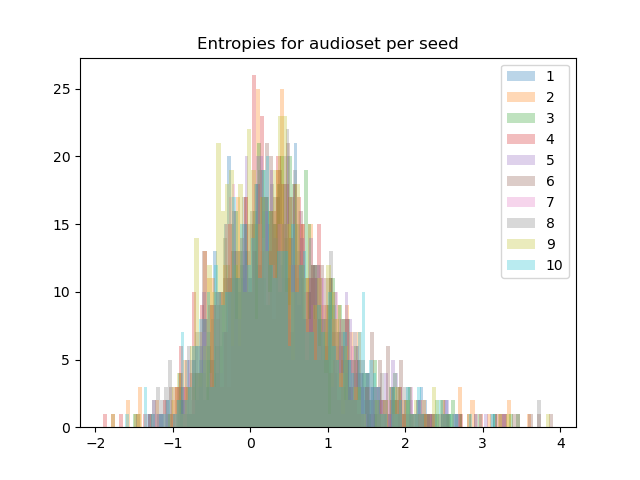
\includegraphics[width=0.45\textwidth]{images/method/probabilistic_independent/audioset_entropies.png}
    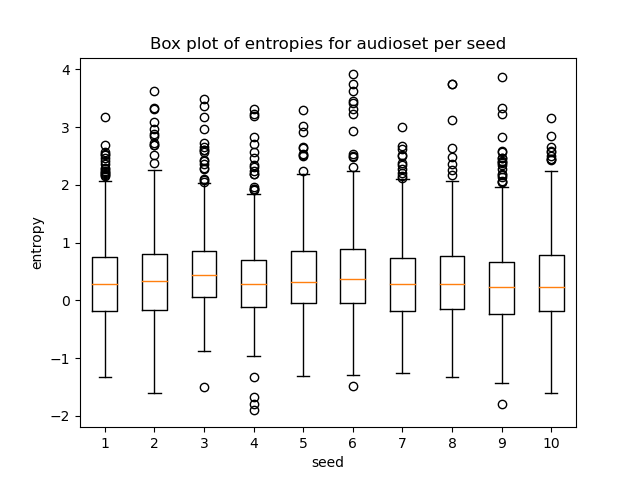
\includegraphics[width=0.45\textwidth]{images/method/probabilistic_independent/audioset_entropies_box.png}
    \caption{
        Histograms of entropy distributions for Open Images and AudioSet embeddings. 
    }
    % generated by analyse.py 
\end{figure}
 
The plots indicate that the distributions of the variances of learned embeddings are stable over different runs. There is more variability in AudioSet graph as there are only 526 concepts versus 19996 in Open Images. The Open Images distribution is bimodal with a very faint peak centered around 7 on the y-axis. 

%\todo[inline]{Add box plots as per JJW comment: "I'd be tempted to produce a sibling graph for each of these two that is a box plot, given that there are a finite number of categories (10).  i.e. put 1 to 10 on the x-axis, and have a box plot for each.  Then it's easy to confirm that the median/quartiles are very similar.  This might especially help with the audio set."}
 
We expect that concepts that occur fewer times should have a higher variance, and therefore higher entropy. This is confirmed by calculating the Spearman correlation of the entropies with the number of incidences of a concept. For AudioSet, this results in a mean Spearman correlation of -0.35 over 10 random seeds, and for Open Images this is a mean of -0.34 over 10 random seeds. 

% audioset
%In [8]: det_learned_corr.mean()
%Out[8]: 0.9189375433154889
%
%In [9]: entropy_count_rcorr.mean()
%Out[9]: 
%spearmanr   -3.465071e-01
%p            7.865913e-14
%dtype: float64


% openimages
%In [5]: det_learned_corr.mean()
%Out[5]: 0.2926545426484884
%In [6]: entropy_count_rcorr.mean()
%Out[6]: 
%spearmanr   -0.336871
%p            0.000000
%dtype: float64


% For the following, run inspect_results.py and call mostalike to dump top 5 neighbours for a few seeds
% then 

\subsubsection{Unexpected clustering behaviour for some concepts depending on hierarchy}

The table below shows the 5 nearest neighbours (in the rows) to the concept ``Cat" in the Open Images domain, over 3 seeds. The metric is Euclidean distance. They do not appear to be very related to the concept of ``Cat".

\begin{table}[H]
\centering
\begin{tabular}{@{}llll@{}}
Rank / Seed &1 &2 &3 \\
\toprule
1&\begin{tabular}[c]{@{}l@{}} Rope \\ 0.290 \end{tabular}&\begin{tabular}[c]{@{}l@{}} Cage \\ 0.257 \end{tabular}&\begin{tabular}[c]{@{}l@{}} Totem pole \\ 0.392 \end{tabular} \\
2&\begin{tabular}[c]{@{}l@{}} Surfing \\ 0.302 \end{tabular}&\begin{tabular}[c]{@{}l@{}} Human \\ 0.306 \end{tabular}&\begin{tabular}[c]{@{}l@{}} Sketch \\ 0.422 \end{tabular} \\
3&\begin{tabular}[c]{@{}l@{}} Hammock \\ 0.302 \end{tabular}&\begin{tabular}[c]{@{}l@{}} Mammal \\ 0.403 \end{tabular}&\begin{tabular}[c]{@{}l@{}} Peace symbols \\ 0.429 \end{tabular} \\
4&\begin{tabular}[c]{@{}l@{}} Picnic table \\ 0.364 \end{tabular}&\begin{tabular}[c]{@{}l@{}} Fawn \\ 0.412 \end{tabular}&\begin{tabular}[c]{@{}l@{}} Beach \\ 0.429 \end{tabular} \\
5&\begin{tabular}[c]{@{}l@{}} Screenshot \\ 0.394 \end{tabular}&\begin{tabular}[c]{@{}l@{}} Vertebrate \\ 0.421 \end{tabular}&\begin{tabular}[c]{@{}l@{}} Outdoor furniture \\ 0.438 \end{tabular} 
\end{tabular}
\centering
% for some reason if there is no caption, the labels get screwed up
\caption{\label{table:cat}The 5 nearest neighbours to the concept ``Cat" in the Open Images domain, over 3 seeds. The distance metric is Euclidean distance.}
\end{table}

However if we examine the same result for a concept that is a more specific instance of ``Cat", we observe much more sensible results for the 5 nearest neighbours. These are the 5 nearest neighbours to the concept ``Domestic short-haired cat" in the Open Images domain, also over 3 seeds. Although this is only a qualitative analysis, we observed the same pattern with the nearest neighbours for other concepts in the Open Images appearing in a hierarchy, for example, ``Human" compared to ``Man" or ``Woman", or ``Jewellery" compared to ``Necklace" or ``Ring". 

\begin{table}[H]
\centering
\begin{tabular}{@{}llll@{}}
Rank / Seed &1 &2 &3 \\
\toprule
1&\begin{tabular}[c]{@{}l@{}} Malayan cat \\ 0.100 \end{tabular}&\begin{tabular}[c]{@{}l@{}} Malayan cat \\ 0.083 \end{tabular}&\begin{tabular}[c]{@{}l@{}} Malayan cat \\ 0.144 \end{tabular} \\
2&\begin{tabular}[c]{@{}l@{}} Burmese \\ 0.195 \end{tabular}&\begin{tabular}[c]{@{}l@{}} Russian blue \\ 0.118 \end{tabular}&\begin{tabular}[c]{@{}l@{}} Himalayan \\ 0.183 \end{tabular} \\
3&\begin{tabular}[c]{@{}l@{}} Russian blue \\ 0.215 \end{tabular}&\begin{tabular}[c]{@{}l@{}} Bombay \\ 0.229 \end{tabular}&\begin{tabular}[c]{@{}l@{}} Russian blue \\ 0.200 \end{tabular} \\
4&\begin{tabular}[c]{@{}l@{}} Abyssinian \\ 0.228 \end{tabular}&\begin{tabular}[c]{@{}l@{}} Polydactyl cat \\ 0.237 \end{tabular}&\begin{tabular}[c]{@{}l@{}} Bengal \\ 0.238 \end{tabular} \\
5&\begin{tabular}[c]{@{}l@{}} Tabby cat \\ 0.240 \end{tabular}&\begin{tabular}[c]{@{}l@{}} Ragdoll \\ 0.256 \end{tabular}&\begin{tabular}[c]{@{}l@{}} Tabby cat \\ 0.267 \end{tabular} 
\end{tabular}
\centering
\caption{\label{table:subclasscat}The 5 nearest neighbours to the concept ``Domestic short-haired cat" in the Open Images domain, over 3 seeds. The distance metric is Euclidean distance.}
\end{table}

Additionally, the most specific terms in the domain often have more meaningful nearest neighbours. For example, these are the 5 nearest neighbours to the concept ``Roti canai", which is a very specific type of Malaysian flatbread. The nearest neighbours are extremely specific and accurate; ``Roti prata", ``Paratha",  ``Naan" and ``Uttapam" are all types of flatbread from different Asian countries. We found many other examples of this phenomenon when inspecting the results. 

\begin{table}[H]
\centering
\begin{tabular}{@{}llll@{}}
Rank / Seed &1 &2 &3 \\
\toprule
1&\begin{tabular}[c]{@{}l@{}} Roti prata \\ 0.222 \end{tabular}&\begin{tabular}[c]{@{}l@{}} Roti prata \\ 0.264 \end{tabular}&\begin{tabular}[c]{@{}l@{}} Roti prata \\ 0.145 \end{tabular} \\
2&\begin{tabular}[c]{@{}l@{}} Tortilla de patatas \\ 0.235 \end{tabular}&\begin{tabular}[c]{@{}l@{}} Roti \\ 0.299 \end{tabular}&\begin{tabular}[c]{@{}l@{}} Pastelón \\ 0.329 \end{tabular} \\
3&\begin{tabular}[c]{@{}l@{}} Pastelón \\ 0.244 \end{tabular}&\begin{tabular}[c]{@{}l@{}} Paratha \\ 0.303 \end{tabular}&\begin{tabular}[c]{@{}l@{}} Timballo \\ 0.340 \end{tabular} \\
4&\begin{tabular}[c]{@{}l@{}} Paratha \\ 0.287 \end{tabular}&\begin{tabular}[c]{@{}l@{}} Uttapam \\ 0.315 \end{tabular}&\begin{tabular}[c]{@{}l@{}} Pastitsio \\ 0.350 \end{tabular} \\
5&\begin{tabular}[c]{@{}l@{}} Timballo \\ 0.360 \end{tabular}&\begin{tabular}[c]{@{}l@{}} Naan \\ 0.358 \end{tabular}&\begin{tabular}[c]{@{}l@{}} Bobotie \\ 0.376 \end{tabular} \\
\end{tabular}
\centering
\caption{The 5 nearest neighbours to the concept ``Roti canai" in the Open Images domain, over 3 seeds. The distance metric is Euclidean distance. }
\end{table}

Embeddings constructed using Euclidean distance measures are known to be less able to represent hierarchical structures, particularly if the embedding space low-dimensional. \cite{NNAnalysisPsychologicalSpaces} found that there is quite a restrictive upper bound on the number of points with the same nearest neighbour when the points lie in Euclidean space. When there is a hierarchical semantic structure to the data, nodes that correspond to more abstract types should have many nearest neighbours. Because of this restrictive upper bound, embeddings learnt in Euclidean space are not able to capture all of these nearest neighbours. \cite{PoincareEmbeddings} describes a method of learning embeddings in hyperbolic space (with constant negative curvature) that may be better able to handle this.

The AudioSet nearest neighbours (not shown here for brevity) for concepts were generally more meaningful. This is probably because as there are only 526 concepts represented in AudioSet, there is less of a hierarchy. 


\section{Alignment}

\subsection{Definition of alignment for this problem}
\label{section:alignmentdef}
As stated in \cite{ManifoldLearningTheoryAndApplications}, the generic alignment problem involves finding a function that maps one domain to the other. This project involves simultaneously learning embeddings for both domains along with the alignment mappings. Since the GloVe algorithm involves stochastic gradient descent over a complex loss surface, it will be highly subject to local minima. Further constraining the problem by inducing alignment should help to decrease the occurrence of local minima and arrive at a better global solution. 

We aim for the type of alignment described in Figure \ref{fig:alignment2}, learning a mapping directly from one domain to another, rather than mapping both domains to an intermediate space because at this stage, we cannot make any assumptions about the manifold that the data lie on. We used 6 dimensions based on previous heuristic analysis.  

For this problem, the $x$- and $y$-embeddings (Open Images and AudioSet respectively) are considered to be aligned if the following holds:

\begin{itemize}
    \item For every member of the set $x_{intersect} = y_{intersect}$ of concepts that exist in both domains, the nearest neighbour of mapped concept $f(x_i)$ is the corresponding member $y_i$ in set $y_{intersect}$, and the nearest neighbour of mapped concept $g(y_i)$ is the corresponding member $x_i$ in set $x_{intersect}$. 
\end{itemize}

The accuracy is computed after each epoch and defined as the fraction of concepts (in the intersection) in a domain whose nearest neighbour after mapping is the known other embedding in the other domain. Accuracy of 1.0 for domain $x$ denotes that for every concept $x_i$ in domain $x$, the nearest neighbour of $f(x_i)$ is $y_i$ where it is known that $x_i$ corresponds to $y_i$. 

\subsection{Model architecture}

This project only aims to prove that the principles are sound, therefore no tuning of architecture or hyperparameters was done. 

We implement, in PyTorch, the following alignment network: 

\begin{itemize}
    \item A probabilistic GloVe embedding layer representing the Open Images embeddings to be aligned (henceforth referred to as the $x$-embeddings). 
    \item A probabilistic GloVe embedding layer representing the AudioSet embeddings to be aligned (henceforth referred to as the $y$-embeddings). 
    \item A multi-layer perceptron with 3 hidden layers of 100 nodes each, that learns a mapping from the $x$-embeddings to the $y$-embeddings: $f(x) \rightarrow y$ 
    \item A multi-layer perceptron with 3 hidden layers of 100 nodes each, that learns a mapping from the $y$-embeddings to the $x$-embeddings: $g(y) \rightarrow x$
\end{itemize}

This particular aligner architecture has been used in previous experiments, with good results. 

\subsubsection{Full loss function}

The full loss function is

\begin{equation}
\label{eq:fulllossfunction}
\begin{split}
L & = L_{glove, x} + L_{glove, y} + L_{cycle, x} + L_{cycle, y} \\
  & + L_{distance, x-intersect} + L_{distance, y-intersect} \\
  & + L_{distsim, x-intersect} + L_{distsim, y-intersect}
\end{split}
\end{equation}

where the individual components are: 

\begin{itemize}
    \item $L_{glove, x}$: The GloVe loss for $x$ as in \ref{eq:gloveloss}. 
    \item $L_{glove, y}$: The GloVe loss for $y$ as in \ref{eq:gloveloss}. 
    \item $L_{cycle, x}$: The cycle consistency loss from x to y: $||g(f(x)) - x||_2$
    \item $L_{cycle, y}$: The cycle consistency loss from y to x: $||f(g(y)) - y||_2$
    \item $L_{distance, x-intersect}$: The distance loss between $f(x)$ and $y$, for only the intersection of concepts: $||f(x_{intersect}) - y_{intersect}||_2$
    \item $L_{distance, y-intersect}$: The distance loss between $g(y)$ and $x$, for only the intersection of concepts: $||g(y_{intersect}) - x_{intersect}||_2$
    \item $L_{distsim, x-intersect}$: An optional distributional similarity measure between $f(x_{intersect})$ and $y_{intersect}$
    \item $L_{distsim, y-intersect}$: An optional distributional similarity measure between $g(y_{intersect})$ and $x_{intersect}$
\end{itemize}

and $x_{intersect}$ and $y_{intersect}$ represent the embeddings of the concepts that exist in both domains. 

\subsubsection{Experimental method}

For 10 random seeds, one run of the alignment model was done without MMD, then another run with MMD. This results in 20 models, 10 for each random seed without MMD and 10 with MMD. 

\subsubsection{Other model parameters}

The hyperparameter choices below were not cross-validated. 

\label{section:otherparameters}
\begin{itemize}
    \item The mini-batch size is 500.
    \item The Adam optimiser is used with a learning rate of 0.01.
    \item 10 samples of each concept embedding are taken for each mini-batch for a total of 5000 points per mini-batch. As the concept embeddings are themselves distributions, this means that we take 10 samples from each. This acts like data augmentation, and was necessary to achieve alignment of above 95\%. If only one sample was used per concept embedding, maximum alignment accuracy was only around 90\%. 
    \item Alignment accuracy is defined as follows: for $x \in x_{intersect}$, the mean number of $i$ such that nearest neighbour of $f(x_i)$ is  $y_i$. For $y \in y_{intersect}$, the mean number of $j$ such that the nearest neighbour of $g(y_j)$ is $x_j$. 
    \item The model is run for 150 epochs; the mean accuracy (over $x$ and $y$) is measured after every epoch and the model is saved if the mean accuracy is greater than the last epoch mean accuracy. Therefore, the final saved model has the embeddings that gave the greatest mean accuracy. 
\end{itemize}


In the next sections, the individual items in the loss are discussed more thoroughly.

\subsection{GloVe loss}
\label{section:gloveloss}
The GloVe loss equation from \cite{pennington2014glove} is restated here:

\begin{equation*}
\begin{split}
L_{glove} &= \sum_i \sum_j f(X_{ij}) (\vecw_i^T \vecw_j + b_i + b_j - \log X_{ij})^2\\
f(x) &= \begin{cases}
(x/x_{max})^{\alpha}\spaced{if} x \le x_{max},\\
1\spaced{otherwise.}
\end{cases}
\end{split}
\end{equation*}

This is a weighted least-squares problem whose solution should be the set of embeddings where the scaled sum of dot products of each pair $\vecw_i$, $\vecw_j$ should approximate the co-occurrence statistics $X_{ij}$. 

Experimentally, it was found that the GloVe loss for the respective domains had to be scaled by the ratio of concepts: there are 19996 Open Images concepts and 526 Audioset concepts, so the $x$ glove loss (Open Images) is multiplied by 19996 / 526. Without this rescaling, the learned embeddings yielded non-sensible results (see Figure \ref{fig:dysfunctional_clusters}). 

\subsection{Cycle consistency}

The cycle-consistency loss relates a domain's embeddings to their reconstruction after mapping to the other domain and back. This uses transitivity to self-supervise training; we want $g(f(x))$ to be close to $x$ and $f(g(y))$ to be close to $y$. 

As stated in \cite{CycleGAN}, simply requiring $f(x)$ to be close to $y$ and $g(y)$ to be close to $x$ is insufficient as overfitting can result in a network being able to map an arbitrary set of inputs to an arbitrary set of outputs. In the CycleGAN implementation of \cite{CycleGAN}, the L1 norm is used, but in this experiment we use the L2 norm as we do not want a sparsity constraint imposed on the embeddings. 

Thus the cycle consistency loss takes the following form:

\begin{equation*}
\begin{split}
L_{cycle} &= E_x ||f(g(x)) - x||_2 + E_y ||g(f(y) - y||_2
\end{split}
\end{equation*}

This loss is also used in other alignment architectures, for example in the MAGAN, \cite{magan} where it is called reconstruction loss. 

\subsection{Distance loss}

This measures how far away the mapped embedding is from the original embedding. This loss represents the semi-supervised component of the algorithm; it is only calculated for the 230 concepts present in both Open Images and AudioSet.

\begin{equation*}
\begin{split}
L_{distance} &= E_{x_{intersect}}||f(x_{intersect}) - y_{intersect}||_2 + E_{y_{intersect}}||g(y_{intersect}) - x_{intersect}||_2
\end{split}
\end{equation*}

The Manifold Alignment GAN (MAGAN \cite{magan}) used this loss to prevent the generators (the mapping MLPs in our model) learning a mapping that simply superimposed the manifolds without actually aligning the points. 

\subsection{Distributional similarity measure}

We want the distributions of $f(x_{intersect})$ and $y_{intersect}$ to be similar, and likewise for $g(y_{intersect})$ and $x_{intersect}$. To be usable as loss functions, a distributional similarity measure should generate a scalar value that is minimised when the distributions are identical. 

\subsubsection{Maximum mean discrepancy}

The maximum mean discrepancy (MMD) statistic is introduced in \cite{MMDGretton} as a difference in feature means of two distributions, where features are obtained by applying a kernel function to the two samples. If the kernel function meets certain conditions, the MMD between samples of two distributions is zero if the distributions are identical. Summarising the full theory that can be found in \cite{MMDGretton}, the following conditions must hold:

\begin{itemize}
    \item The kernel must be characteristic: If the inputs are random variables $X$ with domain $\Omega$ and distribution $P$, there is a one to one mapping between the mean value in feature space and the distributions. \cite{KernelMeanEmbeddingReview} 
    \item That is, each distinct value for the mean in feature space maps to a different possible distribution. 
    \item Intuitively, the kernel function must be "rich enough" to represent all possible distributions. A known characteristic kernel function that is commonly used is the Gaussian kernel function $k(\vecx, \vecy) = \exp(-\alpha ||\vecx - \vecy||_2^2)$, and this is what we use in our experiments. 
\end{itemize}

Given the following:

\begin{itemize}
    \item $\vecx_i$ are $m$ samples from one distribution  $X$
    \item $\vecy_j$ are $n$ samples from the other distribution $Y$
    \item $k(\vecx, \vecx')$ is a characteristic kernel function
\end{itemize}

The empirical unbiased MMD statistic is as follows:

\begin{equation*}
\label{eq:mmd}
\begin{split}
MMD (k, \vecx, \vecy) &= \frac{1}{m(m-1)} \sumim \sum_{j \neq i}^m k(\vecx_i, \vecx_j) + \frac{1}{n(n-1)} \sumin \sum_{j \neq i}^n k(\vecy_i, \vecy_j) \\
&- \frac{2}{mn} \sumim \sumjn k(\vecx_i, \vecy_j)
\end{split}
\end{equation*}

This is the sum of the within-distribution similarities, less the sum of the cross-distributional similarities. 

%(Can include more items described in http://ssa.cf.ac.uk/big-data/slides/Gretton-MMD-TrainingNetworks.pdf)

The implementation from the \texttt{torch-two-sample} \footnote{\texttt{https://torch-two-sample.readthedocs.io}} library \cite{torchtwosample} was used.

$\alpha$ of 0.01 was used for both domains. This value was chosen because it is close to $\frac{1}{2 \sigma^2}$ where $\sigma$ is the median of the pairwise distances, which is a good heuristic for convergence \cite{Garreau2017LargeSA} .  

